\begin{abstract}
As the complexity and number of data feeds grow, data quality emerges as one of the chief challenges.  Hadoop Inspector
is a data quality and health analyzer intended to dramatically improve the quality and manageability of Hadoop
environments.

Hadoop Inspector can be scheduled to periodically scan an environment with user-supplied checks:  either violations of
rules or warnings of anomalies - at the table and field level. Data Quality checks include: uniqueness, foreign key,
format, or unknown value constraints.  Consistency checks include: row and spot-checking base table row counts against
aggregate tables, peer tables in other clusters, or sources tables.   Policy checks include: existence, age, or table
naming conventions.   The test runner is aggregate-aware so that checking can be performed incrementally and frequently.

Both rule and warning violations can be viewed through a web interface to examine the current integrity of the cluster,
as well as the historical integrity with time series graphs. The current state of the project exists primarily as a
demonstration of the concept, providing a basis for the next steps of completing the test runner, user-check
repositories, UI and packaged-set of reusable tests.

Submitted on August 14, 2015 for the Cloudera Strata Competition.
\end{abstract}

\section{Motivation}
Data quality problems have plagued analytical systems for twenty years: continually appearing in the top four reasons
for project failure. In this space data quality problems loom large - a small defect that could be safely ignored or
forgotten in the transactional world hamper queries and cause users to question our credibility for months.

The advent and innovation in Big Data and Data Science has not diminished this challenge. On Hadoop specifically:

\begin{easylist}[itemize]
    @ Our data generally lacks any enforced constraints to ensure data validity
    @ We are adding data faster than ever, with less time to research upstream and ETL pipeline issues
    @ We are building vast systems, sometimes with hundreds of thousands of tasks being defined
    @ We often have democratized access to our clusters - with dozens of different people adding data.
\end{easylist}

Additionally, in these large clusters most teams struggle to comply with policies and other requirements, whether
regulatory, corporate or defined by their own teams. These might define general data retention requirements, or specific
requirements for individual tables. They might define table naming conventions, security requirements, or stats aging \&
collection requirements.


\section{Objective}
Hadoop-Inspector is being built because we believe that the complexity of a large, constantly loaded cluster defies an
unmanaged approach or QA testing in the development process. It requires something more like an automobile assembly
line: continuous quality control (QC) that can take into account undocumented changes from upstream sources, accidental
changes to production, changes that bypass QA, etc. And it shouldn't be limited to traditional quality tests, but should
be able to test for compliance with policies as well.


\section{Technical Details}
Users determine the schedule on which they wish to test their cluster, and every allotted time increment, every check
is run. These results are kept in a local database which is then referenced when users examine the frontend.

Again, given the intricacies of a hadoop cluster, most checks should be written by the cluster maintainers and
operators. Every environment and system is different, and every cluster will have different requirements. We've strived
to provide some basic checks, as well as suggestions for checks that may apply to cluster-specific requirements, however
for the most part, these checks are the user's responsibility.

    \subsection{Checks}
    Every check is simply a script that lives in a type-specific folder. Rules and Warnings exist separately. The directory
    structure is up to the user, however we recommend using our standard layout:

    \begin{verbatim}
    checks
        |--Rules
        |--Warnings
    \end{verbatim}

    The final directory structure is configurable through either JSON config, or command-line arguments.

    Each script returns a JSON-encoded object to {\ttfamily stdout} that meets the following specification. Every check
    that is added to the system must abide by this specification in order to be added to the record. If a check does
    not meet this specification its output will be ignored.

    \begin{minted}{json}
    {
        "name":"Name of test",
        "violations":9000,
        "Output":"Test Specific output. Either JSON or String"
    }
    \end{minted}

        \subsubsection{Rules}
        Rules are strict rules about the cluster. They should never be ignored, or disobeyed, and any violation of a set rule
        results in a violation. Ideally, a ``healthy'' cluster should have no rule violations.

        An example rule would be that a specific column only contains integers.

        \subsubsection{Warnings}
        Checks are suggestions about specific tables, or databases. These are a lot more fluid, and a warning from a check does
        not necessarily indicate an issue with the database, but rather that something new may have happened.

        For example, a check that examines the average number of a column may throw a warning if an entry is too far from the
        mean. This isn't an indication that the data is bad, just that it \textit{may} be bad.

    \subsection{Viewing Results}
    All results can be viewed through the front end. This provides a way to analyze your cluster's health, as well as its
    current status.

    \begin{figure}[H]
        \centering
        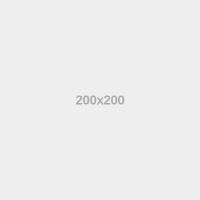
\includegraphics[scale=0.2]{./img/index.png}
        \caption{Index}
    \end{figure}

    \begin{figure}[H]
        \centering
        \includegraphics[scale=0.2]{./img/prod.png}
        \caption{Environment View}
    \end{figure}

    \begin{figure}[H]
        \centering
        \includegraphics[scale=0.2]{./img/westwind.png}
        \caption{Database View}
    \end{figure}

    \subsection{Configuration}
    Most aspects of this framework can be configured using the JSON files located in {\ttfamily /config}. As of \today,
    the files are located in {\ttfamily /config}.

\section{Current Status}
Our initial focus has been on building a demo to help us validate ideas, and build some of our UIs. This includes:

\begin{easylist}[itemize]
    @ \textbf{hadoopinspector-demogen -} Can generate $50,000+$ check results against a hypothetical user hadoop environment
    @ \textbf{server -} Runs a website that allows the user to analyze these demo results
    @ \textbf{report -} Produces a pdf check result summary report
\end{easylist}

